\documentclass{article}

%for graphics
\usepackage{pgfplots}
\pgfplotsset{compat=1.10}

%paragraph formatting
\setlength{\parindent}{0pt}
\setlength{\parskip}{1em}


\begin{document}

\title{Track Forever Initial Results}
\date{\today}
\author{ Christopher Addison (cjteam) \\
         William Cao (pastor13) \\
         David Dupre (djdupre) \\
         Jared Le (jaredtle) \\
         Christine Ta (cta95) }
\maketitle


\section{Introduction}
    The following report has been automatically generated. Its purpose is to provide 
    illustrations of the effectiveness of Track Forever. In order to generate these results, 
    several projects were selected from public issue trackers and imported into Track Forever. 
    At this point, issues were manually evaluated according to the following rubric.

    \begin{center}
        \renewcommand{\arraystretch}{1.5}
        \begin{tabular}{ p{6cm} | c | l }
        Test & Weight & Pass/Fail \\ \hline
        Was important information preserved (Not including user information)? & 2 & Yes/No \\
        Are there any visible errors in the final converted text? & 1 & Yes/No \\
        Can the submitter, commenter, and assignees all be identified (if they exist)? & 1 & Yes/No \\
        Is the issue readable? & 1 & Yes/No \\
        \end{tabular}
    \end{center}

    This part must be done manually. Quality of the conversion is a measurement that only humans can make.

    For each issue evaluated, the results from the rubric were written into a CSV file. 
    An automated script then tabulated the results and generated this report.\pagebreak\section{Issue Tracker GitHub : Project Microsoft DotNet}
\textbf{Conversion Quality Test}
\begin{center}
	\renewcommand{\arraystretch}{1.5}
	\begin{tabular}{ p{6cm} | c | l }
		Test & Weight & Pass/Fail \\ \hline
		Was important information preserved (Not including user information)? & 2 & 0.50 \\
		Are there any visible errors in the final converted text? & 1 & 0.50 \\
		Can the submitter, commenter, and assignees all be identified (if they exist)? & 1 & 0.50 \\
		Is the issue readable? & 1 & 0.47 \\
	\end{tabular}
\end{center}
Final Score for issue tracker: 2.47 / 5.00 \\ \\	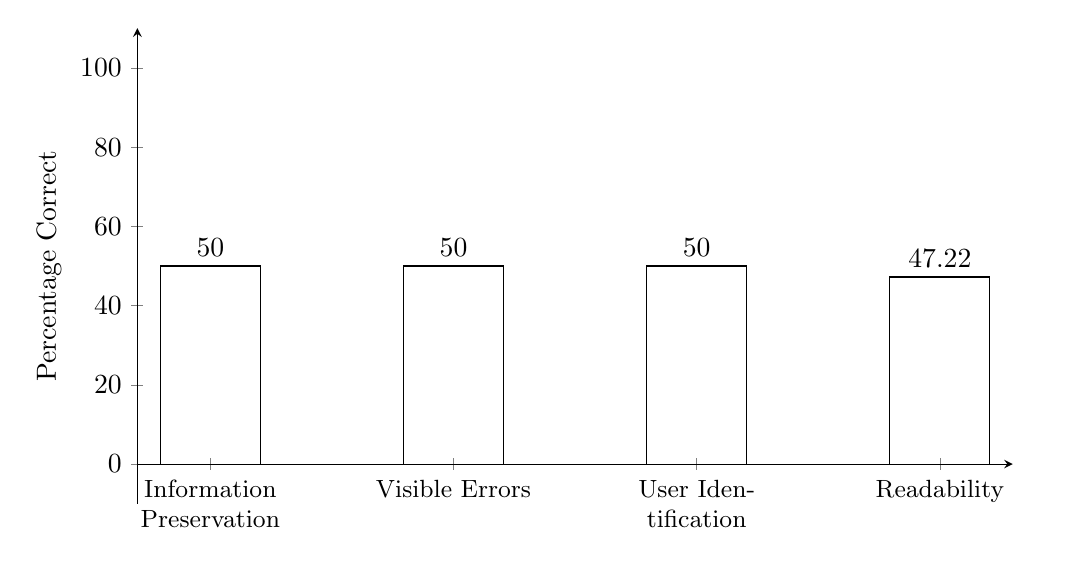
\begin{tikzpicture}
	\begin{axis}[
	width=5in,
	height=3in,
	bar width=0.5in,
	axis x line=center,
	axis y line=left,
	enlargelimits=true,
	ymin=0,
	ymax=100,
	nodes near coords,
	ylabel style={align=center},
	ylabel={Percentage Correct},
	x tick label style={font=\small,text width=1in,align=center},
	symbolic x coords={Information Preservation,Visible Errors,User Identification,Readability},
	xtick=data]
	\addplot[ybar] coordinates {
		(Information Preservation,50.00)
		(Visible Errors,50.00)
		(User Identification,50.00)
		(Readability,47.22)
	};
	\end{axis}
	\end{tikzpicture}\pagebreak\section{Issue Tracker GitHub : Project Minecraft Forge}
\textbf{Conversion Quality Test}
\begin{center}
	\renewcommand{\arraystretch}{1.5}
	\begin{tabular}{ p{6cm} | c | l }
		Test & Weight & Pass/Fail \\ \hline
		Was important information preserved (Not including user information)? & 2 & 0.83 \\
		Are there any visible errors in the final converted text? & 1 & 0.79 \\
		Can the submitter, commenter, and assignees all be identified (if they exist)? & 1 & 1.00 \\
		Is the issue readable? & 1 & 1.00 \\
	\end{tabular}
\end{center}
Final Score for issue tracker: 4.45 / 5.00 \\ \\	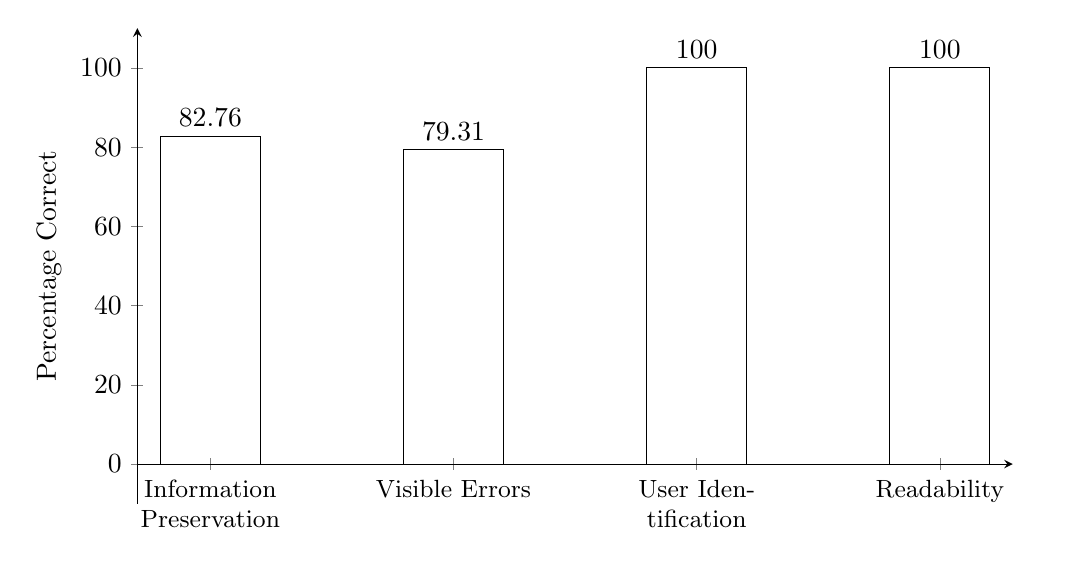
\begin{tikzpicture}
	\begin{axis}[
	width=5in,
	height=3in,
	bar width=0.5in,
	axis x line=center,
	axis y line=left,
	enlargelimits=true,
	ymin=0,
	ymax=100,
	nodes near coords,
	ylabel style={align=center},
	ylabel={Percentage Correct},
	x tick label style={font=\small,text width=1in,align=center},
	symbolic x coords={Information Preservation,Visible Errors,User Identification,Readability},
	xtick=data]
	\addplot[ybar] coordinates {
		(Information Preservation,82.76)
		(Visible Errors,79.31)
		(User Identification,100.00)
		(Readability,100.00)
	};
	\end{axis}
	\end{tikzpicture}\pagebreak\section{Issue Tracker Google Code : Project Appscale}
\textbf{Conversion Quality Test}
\begin{center}
	\renewcommand{\arraystretch}{1.5}
	\begin{tabular}{ p{6cm} | c | l }
		Test & Weight & Pass/Fail \\ \hline
		Was important information preserved (Not including user information)? & 2 & 0.27 \\
		Are there any visible errors in the final converted text? & 1 & 0.52 \\
		Is the issue readable? & 1 & 0.38 \\
	\end{tabular}
\end{center}
Final Score for issue tracker: 1.44 / 4.00 \\ \\	\begin{tikzpicture}
	\begin{axis}[
	width=5in,
	height=3in,
	bar width=0.5in,
	axis x line=center,
	axis y line=left,
	enlargelimits=true,
	ymin=0,
	ymax=100,
	nodes near coords,
	ylabel style={align=center},
	ylabel={Percentage Correct},
	x tick label style={font=\small,text width=1in,align=center},
	symbolic x coords={Information Preservation,Visible Errors,Readability},
	xtick=data]
	\addplot[ybar] coordinates {
		(Information Preservation,27.27)
		(Visible Errors,51.52)
		(Readability,37.88)
	};
	\end{axis}
	\end{tikzpicture}\pagebreak\section{Issue Tracker Google Code : Project OpenBookProject}
\textbf{Conversion Quality Test}
\begin{center}
	\renewcommand{\arraystretch}{1.5}
	\begin{tabular}{ p{6cm} | c | l }
		Test & Weight & Pass/Fail \\ \hline
		Was important information preserved (Not including user information)? & 2 & 0.03 \\
		Are there any visible errors in the final converted text? & 1 & 0.03 \\
		Is the issue readable? & 1 & 0.03 \\
	\end{tabular}
\end{center}
Final Score for issue tracker: 0.14 / 4.00 \\ \\	\begin{tikzpicture}
	\begin{axis}[
	width=5in,
	height=3in,
	bar width=0.5in,
	axis x line=center,
	axis y line=left,
	enlargelimits=true,
	ymin=0,
	ymax=100,
	nodes near coords,
	ylabel style={align=center},
	ylabel={Percentage Correct},
	x tick label style={font=\small,text width=1in,align=center},
	symbolic x coords={Information Preservation,Visible Errors,Readability},
	xtick=data]
	\addplot[ybar] coordinates {
		(Information Preservation,3.45)
		(Visible Errors,3.45)
		(Readability,3.45)
	};
	\end{axis}
	\end{tikzpicture}\pagebreak\section{Issue Tracker Google Code : Project OpenBookProject (Ignoring Import Errors)}
\textbf{Conversion Quality Test}
\begin{center}
	\renewcommand{\arraystretch}{1.5}
	\begin{tabular}{ p{6cm} | c | l }
		Test & Weight & Pass/Fail \\ \hline
		Was important information preserved (Not including user information)? & 2 & 0.99 \\
		Are there any visible errors in the final converted text? & 1 & 0.95 \\
		Is the issue readable? & 1 & 1.00 \\
	\end{tabular}
\end{center}
Final Score for issue tracker: 3.92 / 4.00 \\ \\	\begin{tikzpicture}
	\begin{axis}[
	width=5in,
	height=3in,
	bar width=0.5in,
	axis x line=center,
	axis y line=left,
	enlargelimits=true,
	ymin=0,
	ymax=100,
	nodes near coords,
	ylabel style={align=center},
	ylabel={Percentage Correct},
	x tick label style={font=\small,text width=1in,align=center},
	symbolic x coords={Information Preservation,Visible Errors,Readability},
	xtick=data]
	\addplot[ybar] coordinates {
		(Information Preservation,98.51)
		(Visible Errors,95.05)
		(Readability,100.00)
	};
	\end{axis}
	\end{tikzpicture}\pagebreak\section{Issue Tracker Redmine : Project Project1}
\textbf{Conversion Quality Test}
\begin{center}
	\renewcommand{\arraystretch}{1.5}
	\begin{tabular}{ p{6cm} | c | l }
		Test & Weight & Pass/Fail \\ \hline
		Was important information preserved (Not including user information)? & 2 & 0.00 \\
		Are there any visible errors in the final converted text? & 1 & 0.00 \\
		Can the submitter, commenter, and assignees all be identified (if they exist)? & 1 & 0.00 \\
		Is the issue readable? & 1 & 0.00 \\
	\end{tabular}
\end{center}
Final Score for issue tracker: 0.00 / 5.00 \\ \\	\begin{tikzpicture}
	\begin{axis}[
	width=5in,
	height=3in,
	bar width=0.5in,
	axis x line=center,
	axis y line=left,
	enlargelimits=true,
	ymin=0,
	ymax=100,
	nodes near coords,
	ylabel style={align=center},
	ylabel={Percentage Correct},
	x tick label style={font=\small,text width=1in,align=center},
	symbolic x coords={Information Preservation,Visible Errors,User Identification,Readability},
	xtick=data]
	\addplot[ybar] coordinates {
		(Information Preservation,0.00)
		(Visible Errors,0.00)
		(User Identification,0.00)
		(Readability,0.00)
	};
	\end{axis}
	\end{tikzpicture}\pagebreak\section{Issue Tracker Redmine : Project Project2}
\textbf{Conversion Quality Test}
\begin{center}
	\renewcommand{\arraystretch}{1.5}
	\begin{tabular}{ p{6cm} | c | l }
		Test & Weight & Pass/Fail \\ \hline
		Was important information preserved (Not including user information)? & 2 & 2.00 \\
		Are there any visible errors in the final converted text? & 1 & 1.00 \\
		Can the submitter, commenter, and assignees all be identified (if they exist)? & 1 & 1.00 \\
		Is the issue readable? & 1 & 1.00 \\
	\end{tabular}
\end{center}
Final Score for issue tracker: 7.00 / 5.00 \\ \\	\begin{tikzpicture}
	\begin{axis}[
	width=5in,
	height=3in,
	bar width=0.5in,
	axis x line=center,
	axis y line=left,
	enlargelimits=true,
	ymin=0,
	ymax=100,
	nodes near coords,
	ylabel style={align=center},
	ylabel={Percentage Correct},
	x tick label style={font=\small,text width=1in,align=center},
	symbolic x coords={Information Preservation,Visible Errors,User Identification,Readability},
	xtick=data]
	\addplot[ybar] coordinates {
		(Information Preservation,200.00)
		(Visible Errors,100.00)
		(User Identification,100.00)
		(Readability,100.00)
	};
	\end{axis}
	\end{tikzpicture}\pagebreak\end{document}